\documentclass[11pt]{article}
\usepackage[a4paper,margin=0.9in]{geometry}
\usepackage[section]{placeins}
\usepackage{array}
\usepackage{graphicx,booktabs,amsmath,amssymb,xcolor,hyperref,tikz,multirow,caption,enumitem}
\usetikzlibrary{arrows.meta,positioning,calc}
\captionsetup{font=small,labelfont=bf}
\setlist{nosep,leftmargin=*}
\hypersetup{colorlinks=true,linkcolor=blue!50!black,citecolor=blue!50!black,urlcolor=blue!50!black}
\input{numbers.tex}
\newcommand{\figdir}{../figures}

\title{\vspace{-1.2em}\textbf{STRIDE: Static-profile Routing with Invariant Dynamics Encoding}\\[2pt]
\large Cross-room few-label WiFi-CSI activity recognition --- CS60055 Hackathon 2}
\author{Anubhav (23EE10091)}
\date{}

\begin{document}
\maketitle
\vspace{-2.5em}

\begin{abstract}\small
We build a fully Python pipeline from raw Nexmon PCAP (Room~A) and amplitude CSV (Room~B) to
room identification, self-supervised representation learning and few-label cross-room activity
recognition. Inspecting the data rather than assuming its format exposed three facts that shape everything
downstream: (i) half of the Room-A packets (sequence number \texttt{0xFFFF}) are narrow-band reports, not 80\,MHz CSI; (ii) both rooms mix
20\,MHz frames into the 80\,MHz CSI stream, at a rate that in Room~B depends on the recording session
(and hence on the activity); (iii) Room~A never yields 150 valid observations per capture, while
Room~B is sampled roughly four times faster. We remove invalid observations with physical criteria that are identical for
both rooms, build windows with one symmetric rule, and decompose log amplitude into a static multipath
profile (used for routing) and a low-rank-denoised dynamic part (used for activity). On the fixed validation
sets, the router identifies the room with accuracy \tOneLonefifty{} (\tOneLone{} from a single observation),
self-supervised pretraining raises the linear-probe macro-F1 well above the handcrafted and random-weight
baselines, and cross-room few-label adaptation reaches a macro-F1 of \headAKtwenty{} (B$\to$A) and
\headBKtwenty{} (A$\to$B) at $K{=}20$. We report what does \emph{not} transfer (SIT vs STAND) and why.
\end{abstract}

\section{Problem understanding}
A deployment in a new room can afford only a few labelled captures. The benchmark has two rooms
recorded with the same BCM4366c0 hardware at 80\,MHz but in different sessions. Task~1 identifies the
room from a $(150,256)$ amplitude window; Task~2 learns a representation without labels; Task~3
recognises the target room's own activities from $K\in\{1,5,10,20\}$ labelled captures each, and the
shared SIT/STAND/WALK activities from the \emph{other} room's labels only. The capture is the atomic unit;
validation is never used for fitting; no metadata (format, file name, length) may act as a feature.
We treat these rules as engineering constraints and enforce them in code (split assertions, a
development-only deployment artefact, random window ids, format discarded before routing).

\section{Data engineering}
\begin{figure}[!htbp]
\centering\scriptsize
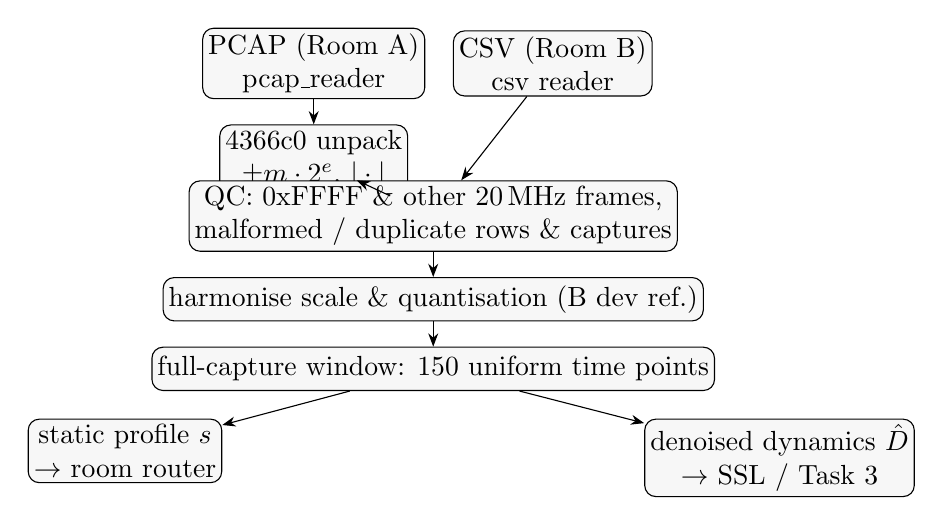
\begin{tikzpicture}[node distance=0.32cm, every node/.style={draw,rounded corners,align=center,
  minimum height=0.55cm,inner sep=2pt,fill=gray!6}, >=Stealth]
\node (a) {PCAP (Room A)\\pcap\_reader};
\node (b) [right=0.35cm of a] {CSV (Room B)\\csv reader};
\node (d) [below=of a] {4366c0 unpack\\$\pm m\cdot2^{e}$, $|\cdot|$};
\node (q) [below=0.32cm of $(d)!0.5!(b)$, yshift=-0.55cm] {QC: 0xFFFF \& other 20\,MHz frames,\\malformed / duplicate rows \& captures};
\node (h) [below=of q] {harmonise scale \& quantisation (B dev ref.)};
\node (w) [below=of h] {full-capture window: 150 uniform time points};
\node (s) [below left=0.35cm and -0.9cm of w] {static profile $s$\\$\to$ room router};
\node (y) [below right=0.35cm and -0.9cm of w] {denoised dynamics $\hat D$\\$\to$ SSL / Task 3};
\draw[->] (a)--(d); \draw[->] (d)--(q); \draw[->] (b)--(q); \draw[->] (q)--(h); \draw[->] (h)--(w);
\draw[->] (w)--(s); \draw[->] (w)--(y);
\end{tikzpicture}
\caption{Pipeline (all stages are our own Python code; the source format only selects the reader).}
\label{fig:pipe}
\end{figure}

\paragraph{Decoding.} We parse classic libpcap records, locate the UDP payload and the Nexmon header
(magic \texttt{0x1111}, sequence, core/stream, chanspec \texttt{0xe02a}=80\,MHz), and unpack each
32-bit BCM4366c0 word as sign/12-bit mantissa for I and Q plus a shared 6-bit exponent, following the
public Nexmon CSI format description~\cite{nexmon} (the authors' MATLAB code was never opened).
Correctness is tested against physics, not against another implementation: synthetic words round-trip,
real spectra are far smoother across adjacent subcarriers than a shuffled order, the 80\,MHz guard
subcarriers (FFT bins 123--133) are deep nulls, and walking varies more over time than standing. Both rooms
turn out to be in the same FFT-bin order.

\paragraph{Three kinds of observation.} Figure~\ref{fig:qc} shows what the inspection revealed.
Room-A reports strictly alternate between a normal sequence number and \texttt{0xFFFF}. The latter lack the
80\,MHz guard nulls and concentrate their energy in the lowest 20\,MHz quarter of the band (median
log-amplitude \insFfffBand{} above the rest of the band), i.e.\ they are narrow-band reports, most likely the other
direction of the ping/pong exchange. Because three quarters of each such row are noise floor, their profile is
dominated by the band mask: it is nearly the same in every capture (mean cross-capture correlation
\insCorrFixed{} versus \insCorrNormal{} for the normal reports) and the median data-subcarrier amplitude is about
\insAmpRatio$\times$ lower. They are not valid 256-subcarrier observations, so we reject them
(\qcArejfixedpattern{} of \qcAndecoded{} decoded reports). Both rooms also contain \emph{narrow-band}
frames whose energy occupies one 20\,MHz quarter of the band; we reject an observation when fewer than
three quarters carry energy (\qcArejpartialband{} in A, \qcBrejpartialband{} in B). This matters beyond
cleanliness: in Room~B such frames make up \insNbSit\,\% of SIT and \insNbStand\,\% of STAND rows, \insNbLying\,\% of
LYING, but only \insNbWalk\,\% of WALK and \insNbEmpty\,\% of EMPTY rows, a session artefact any model would happily learn as an ``activity'' cue. A
byte-identical duplicate capture in the TA package (\texttt{stand65(1).pcap}) is removed by content hash.

\begin{table}[!htbp]
\centering\scriptsize
\caption{Quality control over all captures (both splits; the same rules are applied to every capture).}
\label{tab:qc}
\begin{tabular}{lrr}
\toprule
 & Room A (PCAP) & Room B (CSV)\\
\midrule
\csname @@input\endcsname tab_qc.tex
\bottomrule
\end{tabular}
\end{table}

\begin{figure}[!htbp]
\centering\includegraphics[width=0.62\textwidth]{\figdir/qc_observation_types.png}
\caption{Median spectral profile of the three observation types in Room A (development data).}
\label{fig:qc}
\end{figure}

\paragraph{Harmonisation and windows.} Decoded Room-A values have an arbitrary power-of-two scale and are
non-integer, whereas Room~B is integer; we rescale each Room-A observation to Room~B's median level
(estimated on Room-B development rows) and round, so neither scale nor quantisation can identify the room.
After QC a Room-A capture holds a median of \qcAvalidmed{} valid observations (maximum \qcAvalidmax{}),
never 150. Room~B is sampled faster: the lag-1 autocorrelation of the dominant motion components of
WALK is \insLagA{} in Room~A (native valid observations) and \insLagBone{} in Room~B, falling to \insLagBfour{}
when Room~B is decimated by four. Our deterministic rule, identical for both rooms, resamples the whole
capture's valid sequence onto 150 uniform time points (timestamps for PCAP, row index for CSV) and rounds
to the integer grid; one window is one complete recorded activity instance. A recorded ablation
(\texttt{scripts/12}) against ``150 consecutive valid rows when available'' gives Task-3 macro-F1
\winFullA/\winFullB{} (full) versus \winConsecA/\winConsecB{} (consecutive) for targets A/B, with shared-class
F1 \winFullShB{} versus \winConsecShB{} on target B. No padding rows exist, so capture length cannot leak through
repetition; every window is traceable to its raw file, SHA-1 and configuration in a provenance manifest.

\paragraph{Splits.} Room~A uses the supplied validation folder. For Room~B, candidates are the files
matching the documented patterns, \texttt{sorted()} and sampled with \texttt{random.Random(42)},
25 per activity (the four non-pattern files, which we verified are not duplicates, go to development).
A stratified 20\,\% of development captures is held out internally for every tuning decision.

\begin{table}[!htbp]
\centering\scriptsize\setlength{\tabcolsep}{4pt}
\caption{Design decisions, the evidence behind them (development data unless stated) and the alternative
we rejected.}
\label{tab:dec}
\begin{tabular}{>{\raggedright\arraybackslash}p{3.3cm}>{\raggedright\arraybackslash}p{7.2cm}>{\raggedright\arraybackslash}p{4.4cm}}
\toprule
Decision & Evidence & Rejected alternative\\
\midrule
Reject seq.\ 0xFFFF reports & energy only in the lowest 20\,MHz quarter; no guard nulls; band-mask profile (corr.\ \insCorrFixed) & keep all packets (as a naive reader would)\\
Reject narrow-band frames & energy in one 20\,MHz quarter; class-dependent share in Room B (session artefact) & keep (gives a spurious SIT/STAND cue)\\
Harmonise Room-A scale \& rounding & B is integer with a fixed level; A is arbitrary-scale float & leave as is (format becomes a room cue)\\
Full-capture windows, both rooms & A never has 150 valid observations; ablation: \winFullB{} vs \winConsecB{} on target B & 150 consecutive rows; padding (leaks length)\\
Low-rank denoising of $D$ & naive motion energy inverted in Room B; +0.12/+0.24 shared F1 (Task 3) & raw $D$\\
Capture-consistency SSL, no reversal & capture = one activity; SIT-DOWN reversed = STAND-UP & time-reversal augmentation\\
Room-wise standardisation + LR head & best mean validation macro-F1 (Table~\ref{tab:abl}) & prototypes; SAPT; balanced OT\\
\bottomrule
\end{tabular}
\end{table}

\section{Method}
\paragraph{STRIDE decomposition.} For a window $A$, $L=\log(A{+}1)$; subtracting each observation's median
over data subcarriers removes the gain; the per-subcarrier median over time is the static profile $s$
(environment, posture, location); the remainder $D$ is the body-motion part. Motion changes many
subcarriers coherently (low rank) whereas noise does not, so we keep only singular components of $D$ above
the Gavish--Donoho optimal hard threshold for unknown noise~\cite{gavish} (parameter-free, per window).
This step proved decisive: in Room~B the naive motion energy (median temporal std of $D$) is \insMeRawSit{}
for SIT and \insMeRawStand{} for STAND (noisy sessions) but only \insMeRawWalk{} for WALK; after denoising
WALK is highest (\insMeDnWalk{} vs \insMeDnSit{}/\insMeDnStand), restoring the physical ordering (Fig.~\ref{fig:dn}).

\begin{figure}[!htbp]
\centering\includegraphics[width=0.62\textwidth]{\figdir/denoise_example.png}
\caption{Dynamic part before and after low-rank denoising for two Room-B development windows. The
noisy STAND session is dominated by incoherent fluctuations that disappear; coherent walking structure stays.}
\label{fig:dn}
\end{figure}

\paragraph{Task 1: router.} An $L_2$-regularised logistic regression on $s$ ($C$ chosen on the internal
hold-out). It works for any window length because $s$ is a median over whatever observations exist.

\paragraph{Task 2: self-supervised encoder.} A 121\,k-parameter 1-D CNN: a $1{\times}1$ ``spectral
mixing'' convolution over the 242 data subcarriers, four dilated depthwise-separable temporal blocks and
mean$\|$std pooling to a 128-d embedding. It is trained with an NT-Xent loss~\cite{simclr} whose positives
are two random time spans of the \emph{same capture} --- the only supervision is capture identity, no
activity or room label. Augmentations: random time span (scale/shift), subcarrier-band and time masking,
jitter; time reversal is deliberately excluded because SIT-DOWN reversed is STAND-UP. Two inputs are
compared: the denoised dynamics $\hat D$ (S) and the gain-normalised log amplitude including the static
profile (S$_{raw}$). Frozen embeddings are scored with a logistic-regression probe fitted on development
windows, against handcrafted features (motion-energy bands, temporal spectrum and autocorrelation of the
dominant motion component, static-profile PCs; on $D$ (H) or $\hat D$ (H$_d$)) and the same CNN with
random weights (R).

\paragraph{Task 3: routed, aligned few-label transfer.} (1) The router selects the target room's label space
and normalisation statistics. (2) Features are standardised per room using unlabelled development windows of
that room (validation never). (3) A class-balanced logistic regression is trained on aligned source
windows of the shared classes plus the $K$ support captures of each target-exclusive class. Variants
(ablations): cosine prototypes~\cite{protonet}; \emph{SAPT} --- statistics estimated only from shared-class
windows (exact in the source, iteratively predicted in the target) to counter the label shift between rooms;
balanced optimal-transport refinement on the unlabelled target pool~\cite{cuturi,ptmap}; self-training; and a
strict tier that uses no unlabelled target data. Hyper-parameters were fixed a priori (no target labels).

\section{Experimental setup}
All headline numbers use the fixed validation windows (150 Room-A, 125 Room-B captures, one window each).
SSL: 60 epochs, batch 128, AdamW, 3 seeds, CPU only. Task~3: 10 nested support episodes
($K{=}1\subset5\subset10\subset20$ distinct development captures per exclusive class) for each encoder
seed; we report mean$\pm$std over runs. Macro-F1 is the headline metric (balanced accuracy also
reported); target-exclusive and shared macro-F1 are computed over the respective classes. The headline
Task-3 configuration (\headVariant{} on \headRep{} features) was chosen by mean validation macro-F1 over
both directions and all $K$; because validation guided this choice, all variants are reported.

\section{Results}
\paragraph{Task 1.} Room accuracy is \tOneLonefifty{} at $L{=}150$, \tOneLfive{} at $L{=}5$ and still
\tOneLone{} from a single observation (Fig.~\ref{fig:t1}). The audit is equally informative: motion energy
alone gives \auDyn{} and a four-number temporal-texture probe gives \auTex, i.e.\ the rooms differ not only
in multipath but in session properties (sampling rate, noise floor), while the quantisation probe is at
\auQuant{} after harmonisation. We therefore read the router as a \emph{recorded-environment} fingerprint (Table~\ref{tab:audit}).

\begin{table}[!htbp]
\centering\scriptsize
\caption{Task 1 audit: room accuracy (validation, $L{=}150$) of the same classifier on different evidence.}
\label{tab:audit}
\begin{tabular}{lc}
\toprule
Features & Accuracy\\
\midrule
\csname @@input\endcsname tab_audit.tex 
\bottomrule
\end{tabular}
\end{table}

\begin{figure}[!htbp]
\centering\includegraphics[width=0.55\textwidth]{\figdir/task1_window_length.png}
\caption{Task 1: room accuracy versus window length (same validation captures).}
\label{fig:t1}
\end{figure}

\paragraph{Task 2.} Table~\ref{tab:t2}: self-supervised pretraining clearly beats both required baselines.
S$_{raw}$, which keeps the static profile, reaches the highest within-room and joint accuracy; removing the
static profile (S) costs Room-A accuracy, confirming that posture and location live largely in $s$. This is
the invariance--discriminability trade-off we anticipated. Zero-shot transfer of a source-room SIT/STAND/WALK
probe to the other room stays low for every representation, which motivates Task~3's alignment.
UMAP plots (Fig.~\ref{fig:umap}) show embeddings separating by room first --- consistent with the Task-1
audit --- and by activity within each room. In the STRIDE-SSL embedding the Room-A WALK windows lie next to
the Room-B WALK windows, forming the bridge between the two room clusters: motion transfers, posture does not.

\begin{table}[!htbp]
\centering\small\setlength{\tabcolsep}{6pt}
\caption{Task 2 linear probe on frozen features (validation macro-F1; mean$\pm$std over 3 SSL seeds).
Last two columns: probe trained on the other room's SIT/STAND/WALK only.}
\label{tab:t2}
\begin{tabular}{lccccc}
\toprule
Representation & Room A & Room B & Joint (8) & B$\to$A sh. & A$\to$B sh.\\
\midrule
\csname @@input\endcsname tab_task2.tex 
\bottomrule
\end{tabular}
\end{table}

\begin{figure}[!htbp]
\centering\includegraphics[width=0.85\textwidth]{\figdir/task3_label_efficiency.png}
\caption{Task 3 label efficiency (validation; mean and 95\,\% CI over seeds$\times$episodes): all classes,
target-labelled (exclusive) classes and transferred shared classes.}
\label{fig:le}
\end{figure}

\paragraph{Task 3.} Table~\ref{tab:t3} and Fig.~\ref{fig:le} give the headline. Target-labelled classes
improve steadily with $K$; transferred shared classes stay well below them. Routing matters
(Fig.~\ref{fig:rout}): with the router the mean macro-F1 is \routPredA{} (target A) and \routPredB{}
(target B) versus \routNoneA{} and \routNoneB{} without routing; predicted and oracle routing coincide
because the router makes no validation errors. The ablation (Table~\ref{tab:abl}) shows (i) aligning room
statistics is essential --- without it no target window is ever assigned a shared class; (ii) the
discriminative head beats prototypes; (iii) SSL features help on Room~B and their combination with
handcrafted features is competitive, but denoised handcrafted features are as strong overall; (iv) SAPT's
shared-anchored statistics and balanced OT improve shared-class F1 for target~A at the cost of exclusive
classes, so they do not win on the combined metric --- our label-shift hypothesis is only partly supported.

\paragraph{Denoising is the largest single gain.} With the headline method and identical handcrafted
features, computing them on the denoised $\hat D$ instead of $D$ raises shared-class F1 from
\dnRawSharedA{} to \dnDenSharedA{} (target A) and from \dnRawSharedB{} to \dnDenSharedB{} (target B),
and overall macro-F1 from \dnRawMacroA{} to \dnDenMacroA{} and from \dnRawMacroB{} to \dnDenMacroB.

\paragraph{Why shared-class F1 falls as $K$ grows.} More support captures make the exclusive classes broader
in feature space; ambiguous target windows of the shared classes, which are only described by the
\emph{other} room's data, are increasingly absorbed by the better-described exclusive classes
(Fig.~\ref{fig:le}). Overall macro-F1 still rises with $K$ because the exclusive classes improve faster.
Per class (Table~\ref{tab:pc}), transfer is best for SIT in target B and worst for STAND and WALK, which are
swapped across rooms (Fig.~\ref{fig:cm}).

\paragraph{What SSL buys.} Within a room, SSL is the best representation by a wide margin (Table~\ref{tab:t2}).
Across rooms, its advantage depends on the input: S$_{raw}$ (static profile kept) transfers poorly, because
it relies on room-specific multipath, while S (denoised dynamics) is the best single representation for
target B. Neither beats denoised handcrafted features on target A, where the source room (B) offers only three
shared classes recorded in noisy sessions.

\begin{table}[!htbp]
\centering\scriptsize\setlength{\tabcolsep}{2.5pt}
\caption{Task 3 headline (\headVariant, \headRep{} features), validation, mean$\pm$std over runs.}
\label{tab:t3}
\begin{tabular}{llcccc}
\toprule
Dir. & Metric & $K{=}1$ & $K{=}5$ & $K{=}10$ & $K{=}20$\\
\midrule
\csname @@input\endcsname tab_task3_main.tex 
\bottomrule
\end{tabular}
\end{table}

\begin{table}[!htbp]
\centering\small\setlength{\tabcolsep}{7pt}
\caption{Task 3 ablation: validation macro-F1 averaged over $K\in\{1,5,10,20\}$ and all runs, shown as
target A / target B. Rows: adaptation variant; columns: frozen features (H = handcrafted on $D$,
H$_d$ = on denoised $\hat D$, S = STRIDE-SSL, S\,+\,H$_d$ = concatenation).}
\label{tab:abl}
\begin{tabular}{lcccc}
\toprule
Variant & H & H$_d$ & S & S\,+\,H$_d$\\
\midrule
\csname @@input\endcsname tab_task3_ablation.tex 
\bottomrule
\end{tabular}
\end{table}

\begin{figure}[!htbp]
\centering\includegraphics[width=0.65\textwidth]{\figdir/task3_routing.png}
\caption{Routing contribution (validation macro-F1).}
\label{fig:rout}
\end{figure}

\begin{figure}[!htbp]
\centering\includegraphics[width=0.66\textwidth]{\figdir/task3_confusion_K5.png}
\caption{Confusion matrices at $K{=}5$ (accumulated over runs, row-normalised); per-class P/R/F1 in
Table~\ref{tab:pc}.}
\label{fig:cm}
\end{figure}

\begin{table}[!htbp]
\centering\scriptsize\setlength{\tabcolsep}{4pt}
\caption{Per-class precision / recall / F1 at $K{=}5$ (headline configuration, accumulated over runs).}
\label{tab:pc}
\begin{tabular}{llccc}
\toprule
Target & Class & P & R & F1\\
\midrule
\csname @@input\endcsname tab_perclass.tex 
\bottomrule
\end{tabular}
\end{table}

\begin{figure}[!htbp]
\centering\includegraphics[width=0.6\textwidth]{\figdir/task2_embeddings.png}
\caption{UMAP of validation embeddings, coloured by room (left) and activity (right). Qualitative only.}
\label{fig:umap}
\end{figure}

\section{Reproducibility and leakage controls}
The repository regenerates every artefact from the raw data with numbered scripts
(\texttt{split\_exp3}, \texttt{10}--\texttt{11} pipeline, \texttt{20}/\texttt{30}/\texttt{31}/\texttt{40} tasks,
\texttt{50}/\texttt{60} figures and report numbers); every table in this report is generated by a script.
Controls enforced in code and tests (18 tests): split disjointness and 25 validation captures per class;
Room-B validation drawn only from the documented filename patterns; windows are exactly $(150,256)$ float32
with no repeated padding rows; window ids are a random permutation (room not recoverable from the id); the
deployment artefact contains development captures only; \texttt{run\_episode.py} is smoke-tested on raw
PCAP and CSV files and writes \texttt{window\_id, room, label, confidence}. Only capture identity is used in
SSL; validation windows are never passed to any \texttt{fit}. The SSL input scale, the harmonisation level,
the handcrafted PCA and all room statistics are fitted on development data.

\section{Discussion and limitations}
\begin{itemize}
\item \textbf{Room vs session.} Rooms differ in sampling rate and noise floor as well as multipath; the
router (and any embedding) exploits all of them. With two rooms we cannot separate environment from session.
\item \textbf{What transfers.} Motion level (WALK vs static) transfers once noise is removed; SIT vs STAND
does not, because posture is encoded mainly in the room-specific static profile. The confusion matrices also
show WALK$\leftrightarrow$STAND swaps across rooms, which we attribute to session noise and to the
Experiment-2 activity zones (WALK was recorded in its own zone~\cite{schafer}).
\item \textbf{Our own pipeline choices} (rejecting 20\,MHz frames, full-capture windows, interpolation of
the $\sim$60 Room-A observations) are justified by measurements but are choices. The Room-B sampling rate
cannot be recovered without timestamps; our factor of about four rests on WALK motion statistics and is
only used descriptively. A full Room-B window therefore spans more time than a Room-A window.
\item \textbf{Protocol.} Results are capture-disjoint, not subject-disjoint, on two rooms only; validation
guided the choice among reported variants, so headline numbers are optimistic validation results, not test
accuracy. The original paper's random 80/20 results are not comparable.
\end{itemize}

\section*{Contribution statement}
Solo group. I set the objectives, made or approved the design decisions, reviewed the code and results, and
committed and submitted the work. The implementation, experiments and report draft were produced with
substantial AI assistance, as disclosed below.

\section*{AI usage}
Claude (Anthropic) was used extensively throughout: inspecting the raw data, proposing and implementing the
pipeline and models, running all experiments, and drafting this report. I directed the work, made or
approved the key decisions, and reviewed the outputs. Every reported number comes from the committed
scripts and can be regenerated from the raw data; none was typed in by hand.

\section*{Software and data}
Dataset: CSI Human Activity, IEEE DataPort~\cite{schafer}. Libraries: NumPy, SciPy, pandas,
scikit-learn, PyTorch, matplotlib, umap-learn~\cite{umap}. Code and reproduction steps: repository README.

\footnotesize
\begin{thebibliography}{9}\setlength{\itemsep}{0pt}
\bibitem{schafer} J.~Sch\"afer, B.~R.~Barrsiwal, M.~Kokhkharova, H.~Adil, J.~Liebehenschel. Human activity
recognition using CSI information with Nexmon. \emph{Applied Sciences} 11(19):8860, 2021; dataset on
IEEE DataPort, ``CSI Human Activity''.
\bibitem{nexmon} F.~Gringoli, M.~Schulz, J.~Link, M.~Hollick. Free your CSI: a channel state information
extraction platform for modern Wi-Fi chipsets. \emph{WiNTECH}, 2019; \url{https://github.com/seemoo-lab/nexmon_csi}.
\bibitem{gavish} M.~Gavish, D.~L.~Donoho. The optimal hard threshold for singular values is $4/\sqrt3$.
\emph{IEEE Trans.\ Inf.\ Theory} 60(8), 2014.
\bibitem{simclr} T.~Chen, S.~Kornblith, M.~Norouzi, G.~Hinton. A simple framework for contrastive learning of
visual representations. \emph{ICML}, 2020.
\bibitem{protonet} J.~Snell, K.~Swersky, R.~Zemel. Prototypical networks for few-shot learning. \emph{NeurIPS}, 2017.
\bibitem{cuturi} M.~Cuturi. Sinkhorn distances: lightspeed computation of optimal transport. \emph{NeurIPS}, 2013.
\bibitem{ptmap} Y.~Hu, V.~Gripon, S.~Pateux. Leveraging the feature distribution in transfer-based few-shot
learning. \emph{ICANN}, 2021.
\bibitem{umap} L.~McInnes, J.~Healy, J.~Melville. UMAP: uniform manifold approximation and projection.
arXiv:1802.03426, 2018.
\end{thebibliography}
\end{document}
